\section{Proposed Architecture}
\label{proposed_architecture_section}

The proposed tentative architecture is shown in Figure \ref{proposed_architecture}. The overall architecture is based on Sutton's Dyna architecture \cite{Sutton1990}, which combined both model-free learning and model-based learning. What is different from Dyna is the way we generate the model of the environment, which is explained in the following subsections.

\begin{figure}[!htb]
\centering
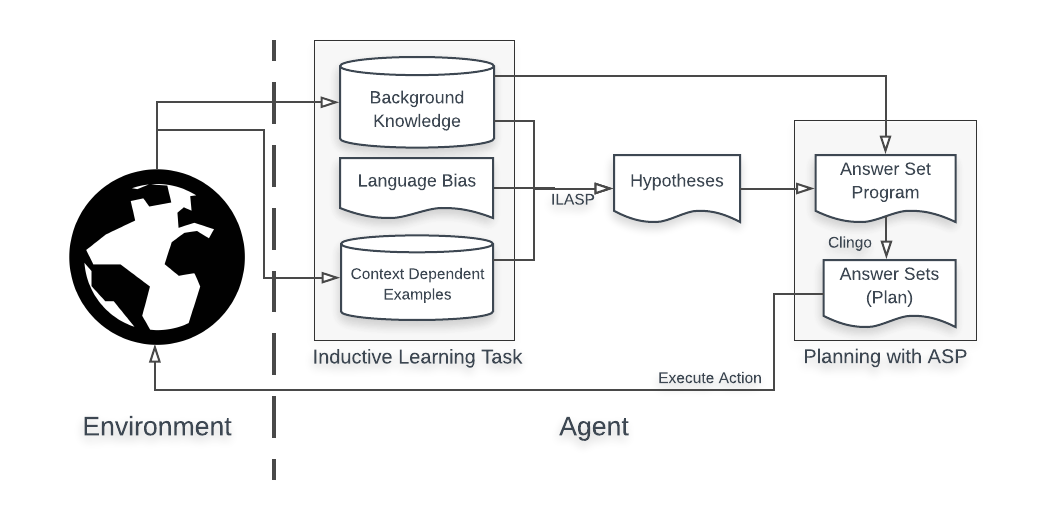
\includegraphics[width=1.0\textwidth]{./figures/architecture}
% 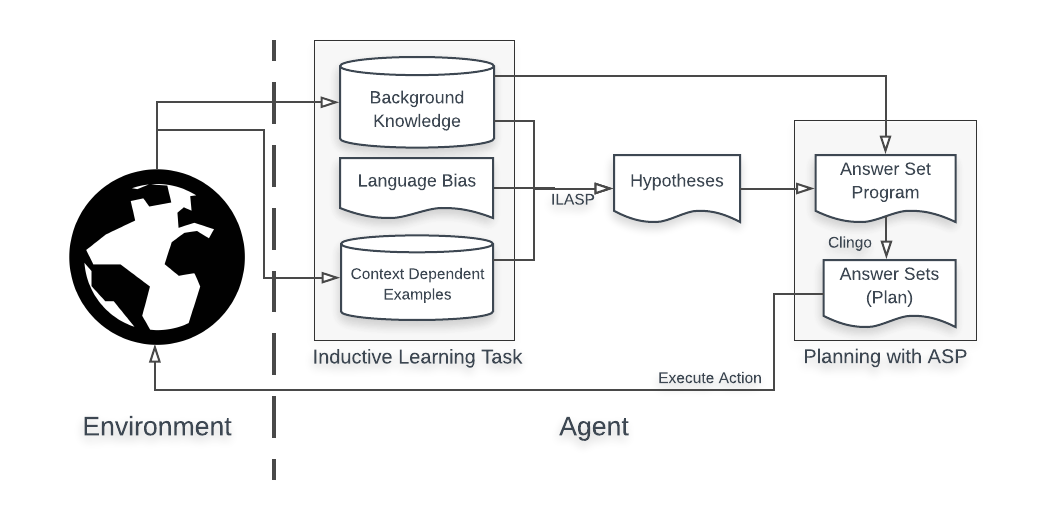
\includegraphics[width=10cm, height=9cm]{./figures/architecture}
\caption{Proposed reinforcement learning architecture. ILASP learns to generate a model and updates based on the interaction with the environment, which is used to facilite the policy evaluation. }
\label{proposed_architecture}
\end{figure}

\subsection{Experience Accumulation}
\label{experience_accumulation}

The first step is to accumulate experience. The agent explores the environment randomly until it reaches the goal once. Until then, it keeps accumulating stuff. 

Every time the agent takes an action, these experiences need to be recorded in two ways: state transition experience and environment experience

State transition experiences will be used as positive examples for ILASP, which is of the form

%\#pos({state_after((X2,Y2))}, {all other state_after that did not happen}, {state_before((X1,Y1)). action(A). }).

For example, 
%\#pos({state_after((3,5))}, {state_after((4,6)),state_after((3,7)),state_after((2,6)),state_after((3,6))}, {state_before((3,6)). action(up). }).

At the first stage,  the input of real experience needs to be converted in ASP form, which can be used to execute the inductive learning in ILASP. The input used in ILASP is state transitions, 
rewards and an action of the agent, which can be directly converted using a simple mapping table or an action language (such as BC\textsuperscript{+} as used in \cite{Ferreira2017}). 
The following ASP input is what is sent to ILASP. \\

agent\_at\_before((X,Y), T).

agent\_at\_after((X,Y), T).

reward(R, T).

action(A, T).

\subsection{Induction}
\label{induction}
Once the agent hits the goal once, ILASP gets triggered and try to learn a hypothesis. 

generate hypothesis H,

later on H should be kept improving as we collect more examples as well as background knowledge.

\subsection{Generate a plan}
\label{Generate a plan}

Generate a plan using abduction

\subsection{Plan execution}
\label{Plan execution}
TODO ALGORITHMS HERE


TODO ALGORITHMS HERE



\subsection{Model Generation and Update using ILASP}
\label{model_generation_and_update}
Once the input of the real experience is converted into ASP syntax, the agent should learn the following definition of the model of the environment using ILASP. \\

valid\_move(C, T):- link(C, T).
\\
link(C2, T):- agent\_at(C1, T), adjacent(C0, C2), not obstacle(C0, C2).\\
%state\_transition(C1, C2, T2):-
%  agent\_at\_before(C1, T1),
%  agent\_at\_after(C2, T2).\\
agent\_at(C, T):- agent\_at\_after(C, T) \\

The background knowledge is empty, and there are only positive examples in learning this task. Each example contains a different transition history of the agent. Inclusions are valid moves and exclusions are invalid moves. Learning valid\_move is the same as learning the rule of the games (the model of the environment), and it is updated as the agent explores in the environment.

In addition to the rules of the game, learning the following concepts will be crucial for transfer learning, as these concepts will be applicable to any types of game environment.  \\

adjacent(C1, C2):- cell(C1), cell(C2). \\
%obstacle(C1, C2):- enemy(C1, C2). \\
obstacle(C1, C2):- wall(C1, C2). \\
wall(C1, C2):- agent\_at\_before(C1, T1), agent\_at\_after(C1, T2) \\
enemy(C1, C2):- agent\_at\_before(C1, T1), agent\_at\_after(C2, T2), reward(R), -100 $\geq$ R \\

where it is assumed that the reward of -100 means losing the game or losing the agent's life. Once the agent has learned the concept of the game, it knows how to avoid an obstacle in an adjacent cell in a new environment. Figure \ref{grid_world} illustrates this transfer capability.



\section{Algorithms}
\label{algorithms}


Once the architecture is decided, we will implement it using Python and ILASPv3.1.0 (Clingo) \cite{Law2017}, and compare the performance with other learning methods using a game platform called GVG-AI Framework.

Other learning methods to be compared as benchmarks will be Q-Learning and Deep Q-Learning since these methods are widely used in other related works. Other symbolic-based approaches could also be compared as an extension. The two main measurements for the performance of our new architecture are learning efficiency and transfer learning capability as stated in the Introduction.

GVG-AI Framework was created for the General Video Gamea AI Competition \footnote{http://www.gvgai.net/}, a game environment for an agent that should be able to play a wide variety of games without knowing which games are to be played.
The underlying language is the Video Game Definition Language (VGDL), which is a high-level description language for 2D video games providing a platform for computational intelligence research (\cite{Schaul2013}).

TODO OPENAI paper citation

The game is formalised as MDP as follows:

\begin{itemize}

\item States: XXX
\item Actions: The agent can move up, down, right or left
\item Rewards: XXX
\item Transitions: XXX

\end{itemize}


% Not sure about this part
\begin{figure}[!htb]
\centering
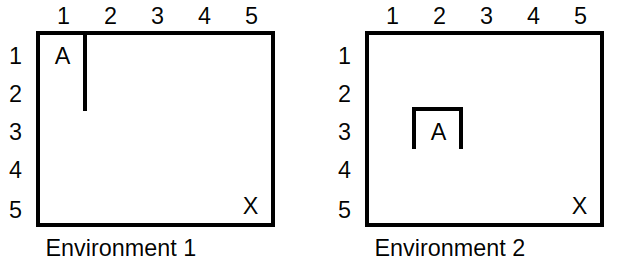
\includegraphics[width=10cm, height=5cm]{./figures/grid_world}
\caption{Simple Grid World to highlight transfer capability }
\label{grid_world}
\end{figure}
If the agent A learnt the concept \textit{adjacent} in Environment 1, the agent could reason (have a policy), for example, "if the adjacent cell is a wall, moving into that cell is an invalid move", "if the adjacent cell is an enemy, moving into that cell will incur a negative reward". These learnt policies could immediately be used in a new environment (e.g Environment 2), even though the agent's coordinates position is different from that in previous environment (e.g Environment 1).
\subsection{Generation of Simulated Experience}
Assuming the model is  a true representation of the partial environment, we can generate simulated experience to update the Q function. The simulated experience is cheaper than real experience, which should contribute to efficient learning. However Dyna architecture is known to lead to sub-optimal policy when the model is not accurate, and the solution to this problem needs to be considered further.

An alternative to using simulated experience is to directly update state representations. Once the concept "adjacent"  was learnt from a real experience, it could be incorporated in a state.

In addition, when the environment changes during the exploration, the agent should generalise its internal model to cope with the new environment in two different but similar environments.  As a result the agent's model becomes more general which covers both games. Thus in theory, the agent should still be able to achieve more efficient learning from the model-based learning, facilitating the transfer learning.
Implementation of exactly how the model is generalised will be further investigated.
